\documentclass[a4paper, 12pt]{report}

\usepackage[finnish]{babel}         % Suomenkielinen tavutus
\usepackage[fixlanguage]{babelbib}
\selectbiblanguage{finnish}
\usepackage[utf8]{inputenc}
\usepackage[T1]{fontenc}
\usepackage{ifpdf}
\usepackage{graphicx}
% load tocbibind package 
%   - do not include table of contents in itself
%   - convert the name of bibliography to references
\usepackage[nottoc]{tocbibind}

% load sverb package
%   - enhanced handling of verbatim stuff; listing environment
\usepackage{sverb}

% load listings package
%   - handle inclusion of source code
\usepackage{listings}
\usepackage{textcomp}
\usepackage{xcolor}

\usepackage{caption}
\usepackage{float}
\usepackage{setspace}
\captionsetup{font={small,stretch=1.1}}

\renewcommand{\lstlistingname}{Listaus}
\lstset{upquote=true,mathescape=false}

% Define JS for listings package
% Source: https://gist.github.com/Geruhn/3d21f60a869457373d84
\definecolor{lightgray}{RGB}{247, 247, 247}
\definecolor{darkgreen}{rgb}{0.0, 0.5, 0.0}
\definecolor{keyword_blue}{HTML}{0141CB}
\lstdefinelanguage{JavaScript}{
  keywords={do, if, for, let, new, try, var, case, else, enum, eval, null, this, true, void, with, await, break, catch, class, const, false, super, throw, while, yield, delete, export, import, public, return, static, switch, typeof, default, extends, finally, package, private, continue, debugger, function, arguments, interface, protected, implements, instanceof, type, of},
  morecomment=[l]{//},
  morecomment=[s]{/*}{*/},
  morestring=[b]',
  morestring=[b]",
  ndkeywords={class, export, boolean, throw, implements, import, this},
  keywordstyle=\color{keyword_blue}\bfseries,
  ndkeywordstyle=\color{darkgray}\bfseries,
  identifierstyle=\color{black},
  commentstyle=\color{darkgreen}\ttfamily,
  stringstyle=\color{red}\ttfamily,
  sensitive=true
}

\lstset{
   language=JavaScript,
   backgroundcolor=\color{lightgray},
   extendedchars=true,
   basicstyle=\linespread{1.1}\footnotesize\ttfamily,
   aboveskip={15pt},
   showstringspaces=false,
   showspaces=false,
   numbers=left,
   numberstyle=\footnotesize,
   numbersep=9pt,
   tabsize=2,
   breaklines=true,
   showtabs=false,
   captionpos=b,
   literate={\$}{{{\$}}}1 {ä}{{\"a}}1 {Ä}{{\"A}}1 {ö}{{\"o}}1 {Ö}{{\"O}}1,
   frame=single
}

% Never insert line breaks in these words:
\hyphenation{JavaScript}
\hyphenation{EcmaScript}
\hyphenation{EcmaScriptin}
\hyphenation{JavaScriptille}
\hyphenation{JavaScriptilla}
\hyphenation{JavaScriptin}
\hyphenation{Closure}
\hyphenation{TypeScript}
\hyphenation{Flow}
\hyphenation{tyypittäminen}
\hyphenation{stan-dar-din}
\hyphenation{VSCode}
\hyphenation{debugattaessa}

% load fancyheaders package
%   - the actual headers and footers are set later
\usepackage{fancyhdr}

% load itpackage 
%   - additional defines and stuff
\usepackage{thesis/itpackage}

\usepackage{enumitem}

\PassOptionsToPackage{hyphens}{url}\usepackage{hyperref}

% Command for inline code, like markdown `code`
\newcommand{\inlinecode}[1]{\colorbox{lightgray}{\texttt{#1}}}

\newcommand{\dblquoted}[1]{\textquotedbl#1\textquotedbl}

\title{JavaScriptin staattinen tyypittäminen}
\author{Oskari Noppa \\kandidaatintutkielma \\ tietojenkäsittelytiede \\ Turun yliopisto}
\date{Lokakuu 2018}

\begin{document}
  \selectlanguage{finnish}\fintrue

  \iffin
  \settocbibname{Lähdeluettelo}
  \renewcommand{\appname}{Liitteet}
  \else
  \settocbibname{References}
  \renewcommand{\appname}{Appendices}
  \fi
  
  % Fill in your information below
  \workinfo{Oskari Noppa}
  {JavaScriptin staattinen tyypittäminen}
  {Jari-Matti Mäkelä}
  {Second Supervisor}
  {2018}
  {10}
  {Lokakuu}
  
  % Set the type of your thesis (Diplomityö, TkK -tutkielma, etc.) and
  % laboratory or field of study below
  \worktype{}{LuK -tutkielma} 
  \deptinfo{}{Tietojenkäsittelytiede}
  
  % Generate the title page 
  \gentitle
  
  % empty pagestyle for table of contents etc. 
  %
  % the redefinition of plain style works also for 1st pages of chapters,
  % which is the default in report class. Just state \thispagestyle{empty}
  % after \chapter{something} if you want empty style for the 1st pages. 
  %
  \pagestyle{empty}
  \fancypagestyle{plain}{
    \fancyhf{}
    \renewcommand{\headrulewidth}{0 pt}
  }
  
  % roman numbering for table of contents etc.
  \pagenumbering{roman}
  
  % insert table of contents, list of figures, list of tables
  %
  % setting the counter to zero effectively removes the page number from
  % the toc, lof etc. entries in the toc since there is no roman numeral
  % for zero ;-) (if you want them without numbering)
  %
  %\setcounter{page}{0}
  \tableofcontents
  \clearpage
  %\setcounter{page}{0}
  %\listoffigures 
  %\clearpage
  %\setcounter{page}{0}
  %\listoftables
  
  % possibly insert 'list of acronyms'
  %
  %   - create a chapter called List Of Acronyms (or whatever), which
  %     should contain all your acronym definitions, e.g. 
  %     \chapter{List Of Acronyms} 
  %   - the secnumdepth trickery is needed because acronyms are as a
  %     standard chapter and we are faking '\listofacronyms'
  %
  %\setcounter{secnumdepth}{-1}
  %\input{your acronym chapter's file name}
  %\setcounter{secnumdepth}{2}
  
  % setup page numbering, page counter, etc.
  \startpages
  
  \chapter{Johdanto} \label{Johdanto}

Ohjelmointi on pohjimmiltaan tietorakenteiden käsittelyä ja yksi tärkeimmistä
tietorakenteen ominaisuuksista on sen tyyppi. Muuttuja “nimi” voi olla
datatyypiltään teksti ja muuttuja “ikä” voi olla numero, eikä näitä kahta voi
huolettomasti sekoittaa. Ohjelman tila ei ole järkevä jos se sanoo henkilön
iän olevan “Matti”. Se miten ohjelmointikielissä käsitellään arvojen tyyppejä
vaihtelee kuitenkin suuresti.

Tässä tutkielmassa käsitellään JavaScriptiä, sekä kolmea työkalua jotka
lisäävät rakentavat staattisesti tarkastettavan tyyppijärjestelmän
JavaScriptin päälle. JavaScript on dynaamisesti tyypitetty ohjelmointikieli,
jonka alkuperäinen käyttötarkoitus oli lisätä verkkosivuille pieniä
interaktiivisia ominaisuuksia, kuten lomakkeiden validointia. JavaScriptillä
toteutettavien ohjelmien koko, monimutkaisuus ja tärkeys on kuitenkin viime
vuosien aikana kasvanut alkuperäistä tarkoitusperää suuremmaksi, kun sillä on
alettu toteuttaa esimerkiksi kartta-, kirjoitus- ja hallintapalveluita jotka
toimivat selaimessa, siten ettei käyttäjän tarvitse asentaa erillistä
ohjelmaa palvelun käyttöön.

Tutkielmassa esitellään TypeScript, Flow ja Closure-kääntäjä, joista jokainen on
kehitetty työkaluksi parempien JavaScript-ohjelmien kehittämiseksi.
Tarkastelussa ilmenee, että staattinen tyypitys voi nopeuttaa ohjelman
kehittämistä, vähentää ohjelmoijan tekemien virheiden määrää ja parantaa
valmiin ohjelman tehokkuutta. Toisaalta nähdään myös, että valinta staattisen
ja dynaamisen tyypityksen välillä sisältää kompromisseja, etenkin kun
tyyppijärjestelmä on erillinen työkalu eikä kieleen alusta asti kehitetty
ominaisuus.

  \chapter{Peruskäsitteitä}

\section{Tyyppijärjestelmien luokitteleminen}
Ohjelmointikielten tyyppijärjestelmien jakaminen staattisesti ja dynaamisesti
tyyppitarkastettuihin perustuu ohjelman kehitysvaiheeseen jossa tarkastaminen
tapahtuu. Staattisella tyyppitarkastamisella viitataan ohjelman tyyppien
analyysiin ennen sen suorittamista, esimerkiksi käännösaikana, kun taas
dynaaminen tyyppitarkastus varmistaa arvojen tyyppien oikeellisuuden ohjelmaa
suoritettaessa. Tyyppijärjestelmät voidaan jaotella myös muiden
ominaisuuksien perusteella, esimerkiksi vahvoihin ja heikkoihin
tyyppijärjestelmiin. Näiden termien merkitys ei ole tarkasti määritelty,
mutta yleisesti niillä viitataan tapaan jolla kieli käsittelee tarkoitetusta
poikkeavat, virheelliset tyypit \cite{CornellTransitionToOO}. Vahvasti
tyypitetyssä kielessä tällainen aiheuttaisi käännös- tai ajonaikaisen
virheen, kun taas heikosti tyypitetyssä kielessä arvoille voitaisiin tehdä
implisiittisiä tyyppimuunnoksia niiden yhteensopivuuden saavuttamiseksi.

JavaScript on dynaamisesti tarkastettu, heikosti tyypitetty kieli.
Esimerkiksi ohjelma \inlinecode{\dblquoted{teksti}.potenssiin(3)} antaa
staattisesti tyyppitarkastetussa kielessä virheen jo käännösaikana, mikäli
metodia \inlinecode{potenssiin} ei ole tekstityyppisille arvoille määritetty.
JavaScriptiä suorittava ympäristö sen sijaan hyväksyisi ohjelman ja sallisi
sen suorittamisen. Virhe olemattoman metodin kutsumisesta ilmenisi vasta jos
ohjelman suoritus evaluoi kyseisen ilmaisun. Lisäksi esimerkiksi ilmaisu
\inlinecode{\dblquoted{teksti} + 2} ei aiheuttaisi virhettä edes 
suoritusaikana, sillä heikoille tyyppijärjestelmille ominaisesti JavaScript
muuttaisi numeron 2 string-muotoon ennen summausoperaation arviointia. Tässä
tutkielmassa keskitytään lähinnä JavaScriptin tyyppien staattiseen ja
dynaamiseen, eli käytännössä käännös- ja ajonaikaiseen tarkastamiseen. Jotkin
esitellyistä työkaluista myös tiukentavat kielen sallimia operaatioita siten,
että esimerkiksi yllä esitettyä \inlinecode{\dblquoted{teksti} + 2} ohjelmaa
ei enää sallittaisi. Monia muita heikoille tyyppijärjestelmille
tavallisia ominaisuuksia jää kuitenkin tarkistamatta.

\begin{figure}
\centering
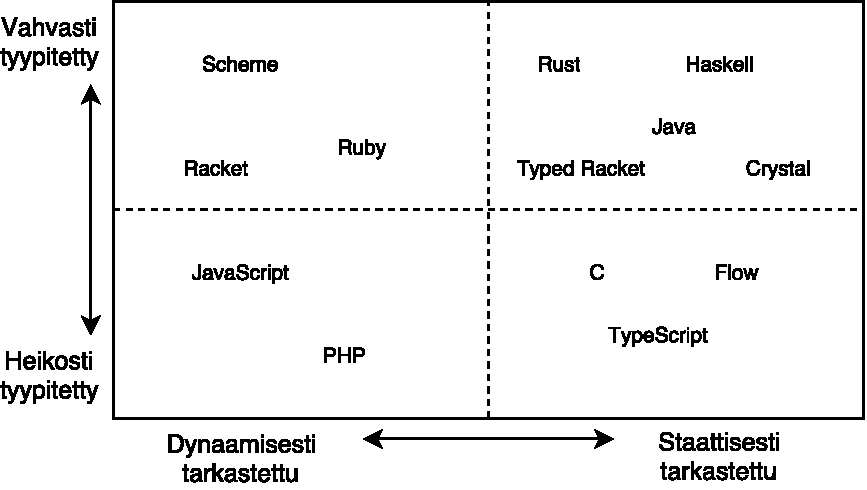
\includegraphics{images/type-systems.pdf}
\caption{Tyyppijärjestelmät eri ohjelmointikielissä}
\end{figure}

\section{ECMA-262, EcmaScript ja JavaScript}
``EcmaScript'' on ECMA-262 standardin määrittelemä ohjelmointikieli
\cite{JavaScriptLanguageResources}\cite{Ecma262}, jonka kehityksestä vastaa
organisaatio Ecma International. ``JavaScript'' on Oraclen omistama
tavaramerkki jolla viitataan EcmaScript-kielen osittaisiin tai täydellisiin
toteutuksiin.[4] Historiallisista syistä termejä
``JavaScript'' ja ``EcmaScript'' käytetään usein keskenään vaihtokelpoisesti.
Tässä tutkielmassa termillä ``JavaScript'' viitataan ECMA-262:den kahdeksannen
version mukaiseen EcmaScriptiin, jota kutsutaan myös nimellä EcmaScript 2017.

\section{TypeScript}
TypeScript on Microsoftin luoma ohjelmointikieli, jonka tarkoitus on
auttaa JavaScript-ohjelmien kehitystä staattisen tyyppijärjestelmän avulla.
Se on EcmaScriptin ylijoukko (superset) \cite{TypeScriptSpec} ja jatkaa
JavaScriptin syntaksia tyyppimäärittelyihin käytettävällä
annotaatiosyntaksilla. Jokainen validi JavaScript-ohjelma on syntaksiltaan ja
ajonaikaiselta käyttäytymiseltään validi TypeScript-ohjelma. TypeScript
kuitenkin lisää kehitykseen käännösvaiheen, jossa ohjelman tyyppien
oikeellisuus tarkastetaan staattisesti. TypeScript koodi käännetään
JavaScriptiksi, joka puolestaan voidaan suorittaa selaimissa tai muissa
JavaScriptin suoritusympäristöissä. TypeScript kääntäjän voi myös määrittää
muokkaamaan tulostettava koodi yhteensopivaksi vanhempien
EcmaScript-standardien kanssa, mikä on hyödyllistä jos ohjelman on tarkoitus
tukea sellaisia suoritusympäristöjä jotka eivät tue uusinta EcmaScriptin
versiota.

\section{Flow}
Flow on Facebookin kehittämä työkalu, joka TypeScriptin tavoin jatkaa
JavaScriptin syntaksia staattisesti tarkastettavilla tyyppimäärittelyillä.
Flow itsessään ei sisällä kääntäjää, vaan keskittyy yksinomaan ohjelman
tyyppiturvallisuuden tarkastamiseen. Koodiin lisätyt tyyppimääritykset on
kuitenkin poistettava ennen kuin JavaScript-ohjelma voidaan suorittaa. Tähän
tarkoitukseen voidaan käyttää esimerkiksi Babel-kääntäjää, joka poistaa
Flow-tyyppimäärittelyt ja muokkaa JavaScript-koodin yhteensopivaksi toivotun
EcmaScript-version kanssa \cite{FlowInstallation}.

\section{Closure kääntäjä}
Googlen Closure kääntäjä on käännöstyökalu, jonka pääasiallinen tarkoitus
on minimoida ja optimoida JavaScript-koodia käännösvaiheessa ennen tuotantoon
siirtämistä. Closure sisältää kuitenkin myös tuen tyyppivirheiden
tarkastamiselle käännösvaiheessa \cite{ClosureCompiler}. Tyypit annotoidaan
erityisellä JSDoc-pohjaisilla dokumentaatiokommenteilla. Koska annotaatiot
ovat kommenteissa eivätkä erityisenä syntaksina muun suoritettavan koodin
joukossa, Closure-annotoitua JavaScriptiä ei tarvitse kääntää ennen sen
suorittamista \cite{annotatingJSforClosure}.
  \chapter{Käyttöönotto}

\section{Tyyppiannotaatiot}

Tyyppijärjestelmä voi päätellä muuttujan sallitun tyypin automaattisesti
tai kielen syntaksin tarjoamien eksplisiittisten tyyppimäärittelyjen
perusteella. Kaikki kolme tässä tutkielmassa esiteltyä JavaScriptin staattiseen
tyyppitarkastukseen tarkoitettua työkalua päättelevät muuttujien tyyppejä
automaattisesti, mutta vaativat paikoitellen myös eksplisiittisiä määrityksiä.
Closure-kääntäjä lukee
tyyppimääritykset JSDoc-tyylisistä dokumentaatiokommenteista \cite{annotatingJSforClosure}.
\begin{lstlisting}[caption={Esimerkki Closure-annotaatiosta funktiolle},label={lst:ostoskorin_hinta_closure}]
/**
* @param {!Array<Ostos>} ostokset
* @return {number} Ostosten yhteenlaskettu hinta
*/
function ostoskorinHinta(ostokset) {
  let summa = 0;
  for (const ostos of ostokset) summa += ostos.hinta;
  return summa;
}
\end{lstlisting}
Listauksessa \ref{lst:ostoskorin_hinta_closure} \inlinecode{ostoskorinHinta}-funktion
tyyppimäärittely on toteutettu sen yläpuolella olevilla kommenteilla, jotka määrittävät
tyypin \inlinecode{ostokset} parametrille sekä funktion palautusarvolle.
TypeScript ja Flow puolestaan jatkavat ECMA-262-spe\-si\-fi\-kaa\-ti\-o\-ta
erityisellä syntaksilla tyyppien eksplisiittistä määrittämistä varten. 
\begin{lstlisting}[
  float,
  caption={Esimerkki Flow tai TypeScript annotaatiosta funktiolle},
  label={lst:ostoskorin_hinta_flow}
]
function ostoskorinHinta(ostokset: Ostos[]): number {
\end{lstlisting}
Flow ja TypeScript -esimerkissä \ref{lst:ostoskorin_hinta_flow}
tyyppiannotaatiot ovat osana koodia, mikä
tekee ohjelmasta yhteensopimattoman tavallisen JavaScriptin kanssa. Ohjelma
on käännettävä JavaScriptiksi ennen suorittamista. Annotaatioiden
syntaksi ja merkitys eivät myöskään ole välttämättä suoraan selviä
JavaScript-ohjelmoijalle, joka pahimmassa tapauksessa voi kokea lisätyt
tyyppimäärittelyt vaikeasti luettavina. 

Closuren annotaatiot on sijoitettu kommentteihin, joten niillä ei ole
ajonaikaista vaikutusta ja ohjelma on täten sellaisenaan hyväksyttävää
JavaScriptiä. Toisaalta tyyppiannotaatioiden määrittely kommenteissa voi
olla runsassanaista ja hankalaa, mikä kasvattaa niiden kirjoittamiseen vaadittua
työmäärää \cite{TypeScriptSpec, TypeScriptatBuild}.

Aiemmassa esimerkissä esitelty tyyppi \inlinecode{Ostos} pitäisi
määritellä Closurea varten muiden annotaatioiden tapaan dokumentaatiokommentteja käyttäen:

\begin{lstlisting}[
  caption={Uuden tyypin määrittely Closuren kommenttisyntaksilla},
  label={lst:closure_typedef}
]
/**
* @typedef {{
*   nimi: string,
*   hinta: number
* }}
*/
let Ostos;
\end{lstlisting}
TypeScript ja Flow tarjoavat käännösaikaisen tyypin (type alias)
määrittelyyn tiiviimmän ja helppolukuisemman syntaksin \cite{TypeScriptSpec}:
\begin{lstlisting}[
  caption={Uuden tyypin määrittely TypeScriptissä tai Flow'ssa},
  label={lst:ts_flow_type_alias}
]
type Ostos = {
  nimi: string;
  hinta: number;
};
\end{lstlisting}
Tällainen tyypin määritteleminen vaikuttaa ainoastaan käännösvaiheen
tyyppitarkastukseen, eikä määrittely tuota tietorakenteita tai muuta
sisältöä suoritettavaan JavaScript-ohjelmaan.

\section{Käännösprosessi}
\begin{figure}[!htb]
\centering
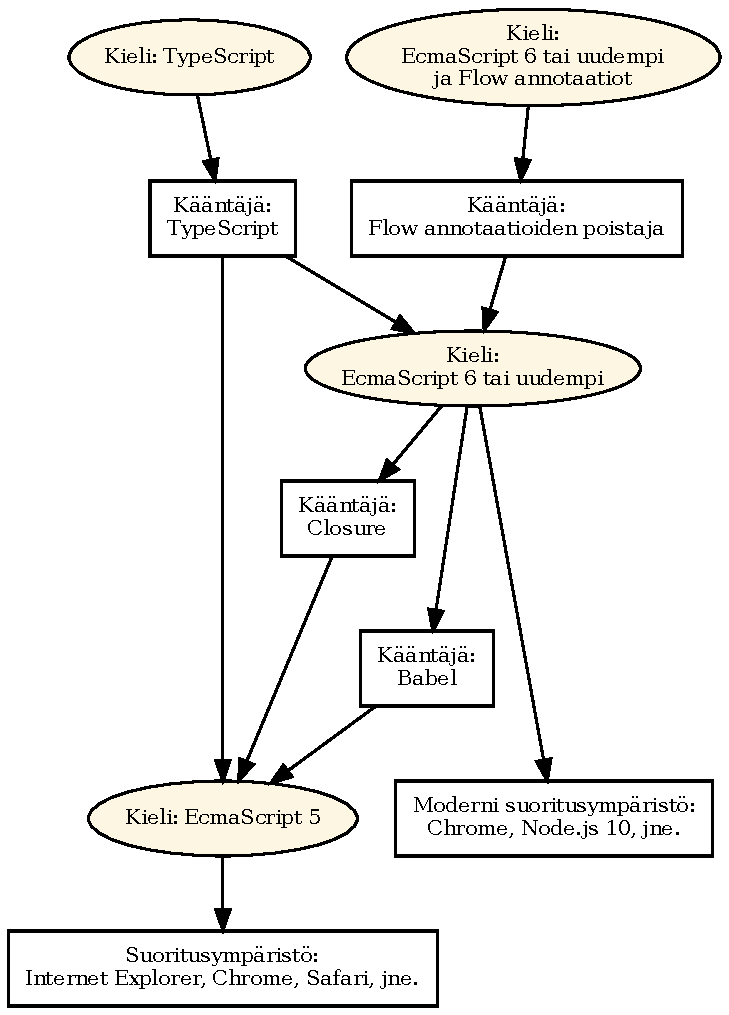
\includegraphics[width=0.8\textwidth]{images/compilation.pdf}
\caption{Vaihtoehtoisia käännösprosesseja}
\label{fig:compilation}
\end{figure}
JavaScriptillä kirjoitettua koodia ei tavallisesti tarvitse
erikseen kääntää ennen suoritusvaihetta. JavaScriptiä suorittava ohjelma,
esimerkiksi selain, tulkkaa EcmaScript-standardin mukaista koodia
sellaisenaan tai \textit{JIT-kääntää} sen optimoituun muotoon automaattisesti
suorituksen ohessa. TypeScript- tai Flow-annotoitu koodi ei kuitenkaan
ole validia JavaScriptiä, eikä selain tai muu JavaScriptia suorittamaan
suunniteltu ohjelma tavallisesti osaa sellaista koodia käsitellä.
Näinollen TypeScript tai Flow-annotoitu koodi on välttämätöntä kääntää muotoon jossa
annotaatiot on poistettu ja jäljellä on enää standardinmukainen JavaScript.

Kääntämisen tarve vaikuttaa ohjelman kehitysprosessiin.
Koska JavaScriptin käyttäminen ei normaalisti vaadi erillistä
käännösvaihetta, useissa projekteissa ei ole sellaista käytetty. Koodin
minimointi ja muu optimointi on ollut parhaiden käytäntöjen mukaista jo
tovin, mutta tällaiset koodinkäsittelyt tehdään yleensä vasta ennen ohjelman
julkaisua. Kehittäjät ovat tavanomaisesti voineet suorittaa kirjoittamansa
JavaScriptin sellaisenaan kehitysympäristössä. Käännösvaiheen aikavaatimus
pyritään luonnollisesti pitämään mahdollisimman pienenä, mutta se on silti
projektin monimutkaisuuteen ja kehitysnopeuteen vaikuttava tekijä, joka
tulee huomioida työkalun käyttöönotossa.

Kuva \ref{fig:compilation} esittää erilaisia käännösprosesseja eri
JavaScript-ohjelman kehityskielille. Käännösvaiheen tarpeellisuus
ja vaikutus kehitysprosessiin riippuu käytetystä kielestä ja sen versiosta,
sekä siitä missä ympäristöissä sitä halutaan suorittaa.
Esimerkiksi Internet Explorer 11 -selain tukee ainoastaan
EcmaScriptin vanhaa viidettä
versiota (2011). Jos koodi kirjoitetaan kaikkiin
suoritusympäristöihin soveltuvalla EcmaScriptin versiolla,
käännösvaihe voidaan jättää kokonaan väliin. Kielen
uudemmat versiot ovat kuitenkin tuoneet monia lisäominaisuuksia,
kuten syntaksin \textit{luokkien} määrittelyyn, joiden
käyttäminen vanhempia selaimia tukevissa ohjelmissa vaatii joka tapauksessa
käännösvaiheen staattisesta tyypittämisestä riippumatta. Uusia
JavaScript-o\-mi\-nai\-suuk\-si\-a hyödyntäville projekteille koodin kääntäminen ei
siis tule täysin uutena vaiheena.

\section{Työkalun vaiheittainen käyttöönotto}

JavaScript-kirjastojen hallintaan tarkoitettu rekisteri \textit{npm} on yksi
suurimmista ohjelmistoekosysteemeistä \cite{DynamicsOfJSPackages}.
Tämän tutkielman kirjoittamisen hetkellä rekisterin kotisivu,\newline
npmjs.com, ilmoitti julkisesti saatavilla olevien pakettien määräksi yli 800 000.
Avoimessa jakelussa olevien kirjastojen lisäksi JavaScriptiä käyttävillä
kehittäjillä voi olla suuri määrä valmista JavaScript-koodia, jota voi
hyödyntää uusissa projekteissa. Jotta TypeScript, Flow ja Closure olisivat
hyödyllisiä työkaluja JavaScript-ohjelmien kehitykseen, on niiden oltava
yhteensopivia sellaisen JavaScript-koodin kanssa jonka kehitykseen ei
kyseistä työkalua ole käytetty.

TypeScript ja Flow tukevat erityisiä määrittelytiedostoja, joiden sisältämällä
tyyppiannotoidulla koodilla määritetään kirjaston tai muun JavaScript-koodin
ulkoisen rajapinnan tyyppimäärittelyt. Näiden tiedostojen kirjoittamiseen
käytetty syntaksi on muuten sama kuin muissakin tiedostoissa, muuta niiden funktio- ja
metodimäärittelyistä on jätetty implementaatiot kokonaan pois. Tiedoston ei
ole tarkoitus olla osana varsinaista suoritettavaa koodia, vaan se palvelee
ainoastaan kuvauksena sellaisen koodin tyyppimäärittelystä, jonka käsittelyä
TypeScript ja Flow eivät muuten voisi valvoa. TypeScriptillä voitaisiin
esimerkiksi kirjoittaa seuraava tiedosto \inlinecode{ostoskori.d.ts}, jonka
tehtävä on annotoida toista tiedostoa \inlinecode{ostoskori.js} (Listaus \ref{lst:tsdfile}).
\begin{lstlisting}[
  caption={Esimerkki TypeScript määrittelytiedostosta ostoskori.d.ts},
  label={lst:tsdfile}
]
export const tuotteet: ReadonlyArray<Ostos>;

/** Lisää tuotteen ostoskoriin. */
export function lisääTuote(ostos: Ostos): void;
\end{lstlisting}
Tämän jälkeen TypeScript tiedostosta käsin voidaan kutsua tätä
JavaScript-funktiota siten, että TypeScript valvoo
tyyppien oikeellisuutta (Listaus \ref{lst:jscallfromts}).
\begin{lstlisting}[
  caption={JavaScript-koodin kutsuminen TypeScript tiedostosta tuotesivu.ts},
  label={lst:jscallfromts}
]
import * as ostoskori from "./ostoskori";

ostoskori.lisääTuote({ nimi: "juusto", hinta: 5 });
// Vääränlainen kutsumistapa aiheuttaisi käännösaikaisen virheen:
ostoskori.lisääTuote('juusto', 5); // Expected 1 arguments, but got 2
\end{lstlisting}
JavaScript-kirjaston kehittäjä voi tarjota erillisen tyypitystiedoston
kirjastonsa lähdekoodin mukana, tai muut kirjastoa käyttävät kehittäjät
voivat oma-aloitteisesti luoda sellaisen tyypitystiedostoja keräävään
julkaisuarkistoon (engl. repository).
TypeScriptin tyy\-pi\-tys\-tie\-dos\-toil\-le
on \textit{DefinitelyTyped} \cite{DefinitelyTyped} ja Flowlle
vastaavasti \textit{flow-typed} \cite{FlowTyped}. Vaikka Flow ja TypeScript
ovatkin monin tavoin hyvin samankaltaisia, eivät ne kuitenkaan ole täysin
yhteensopivia. Yhdelle tyyppijärjestelmälle luotuja annotaatiotiedostoja
ei siis yleensä voi suoraan käyttää toisella järjestelmällä, joskin niiden
muuntaminen toisen tyyppijärjestelmän käytettäväksi on useimmiten melko
suoraviivaista ja ainakin osin automatisoitavissa työkaluilla kuten
\textit{flowgen} (TypeScript-tyypitykset Flow-tyypityksiksi) \cite{Flowgen},
\textit{clutz}  (Closure-tyypitykset TypeScript-tyypityksiksi) \cite{Clutz}
ja \textit{tsickle} (TypeScript-annotoitu koodi Closure-annotoiduksi) \cite{Tsickle}.
Joitain perustavanlaatuisia eroja työkalujen välillä voi silti olla vaikea
tai mahdotonta siirtää tyyppijärjestelmästä toiseen tekemättä kompromisseja.
TypeScriptissä esimerkiksi kaikki \textit{enumeja} lukuunottamatta on
\textit{rakenteellisesti} (engl. structural) tyypitetty, kun taas Flow'ssa 
esimerkiksi luokkien instanssien tyyppejä vertaillaan \textit{nimellisesti}
(engl. nominal), mikä aiheuttaa tyyppijärjestelmien käyttäytymisessä eroja
jos jotkin kaksi luokkaa ovat rakenteeltaan täysin samat. Tämän tutkielman
viimeisestä luvusta löytyy esimerkki \ref{fig:structural_typing_error}
juuri tällaisesta tilanteesta; siinä luokat \inlinecode{Ihminen} ja
\inlinecode{Eläin} ovat rakelteeltaan samanlaisia ja käsitellään siksi
TypeScriptissä kuin ne olisivat sama luokka, mutta Flow'ssa kahtena
erillisenä luokkana jotka eivät ole keskenään vaihtokelpoisia. 

Joissain tapauksissa kirjastoille tai kehittäjän omalle aiemmin kirjoitetulle
JavaScript-koodille ei kuitenkaan ole valmiita TypeScript-tyyppimäärittelyjä
eikä niitä syystä tai toisesta voida luoda ennen muun kehityksen jatkamista.
JavaScript-kirjaston rajapinta voi olla liian iso tyypitettäväksi projektin
aikatauluun sopivalla tahdilla, tai se saattaa olla suunniteltu käyttämään
sellaisia dynaamisia JavaScriptin ominaisuuksia joita ei helposti voida
tyypittää TypeScriptin, Flown tai Closuren tarjoamalla tyyppijärjestelmällä.
Kaikkien kolmen työkalun tärkeimpiin ominaisuuksiin kuuluu tuki vaiheittaiselle
käyttöönotolle, eli käytännössä yhteenspivuus täysin tyyppitarkastamattoman
koodin kanssa.

Sekä Flow että TypeScript tarjoavat erityisen
yleisviittaustyypin Any, jota voi käyttää kuvaamaan mitä tahansa
JavaScript-arvoa \cite{TypeScriptSpec}. Any-tyyppiseen muuttujaan voidaan asettaa mikä
tahansa arvo ja Any-tyyppinen arvo voidaan asettaa mihin tahansa muuttujaan
tai funktioparametriin. Any-tyypin avulla muuten staattisesti tyypitetyssä
ohjelmassa voidaan ohittaa käännösaikainen tyyppien tarkistaminen sellaisten
koodin osien kohdalla joiden ajonaikaista arvoa olisi muuten vaikea tai
mahdotonta määritellä käännösaikana. Näin ollen, mikäli tarve vaatii täysin
annotoimattoman JavaScript-moduulin käyttämistä, kaikkien kyseisestä moduulista
tuotujen arvojen voidaan määrittää olevan tyyppiä Any, jolloin tarkastaja ei
kiinnitä huomiota siihen miten JavaScriptillä määritettyjä funktioita tai
muita arvoja käsitellään.
\begin{lstlisting}[
  caption={Esimerkki Any-tyypillä sivuutetusta TypeScript virheestä},
  label={lst:tsany}
]
const koriElementti: null | HTMLElement =
  document.getElementById('kori')
// Tiedetään että elementti on dokumentissa eikä null.
const koriElementtiEiNull: HTMLElement = koriElementti as any
koriElementtiEiNull.innerHTML = '<h1>Ostoskori</h1>'
\end{lstlisting}
Esimerkin \ref{lst:tsany} \inlinecode{getElementById}-funktiokutsu
palauttaisi \inlinecode{null} jos kori elementtiä ei löytyisi dokumentista,
mutta virhe on päätetty ohittaa määrittämällä eksplisiittisesti
muutujan tyypiksi ensin \inlinecode{any} ja sitten \inlinecode{any} tyypistä
\inlinecode{HTMLElement} tyypiksi. Flow sallii tyyppivirheiden sivuuttamisen
myös erityisillä kommenteilla.
\begin{lstlisting}[
  caption={Esimerkki kommentilla sivuutetusta Flow virheestä},
  label={lst:flowignore}
]
const koriElementti: null | HTMLElement =
  document.getElementById('kori')
// $FlowFixMe Tiedetään että elementti on dokumentissa eikä null.
const koriElementtiEiNull: HTMLElement = koriElementti
koriElementtiEiNull.innerHTML = '<h1>Ostoskori</h1>'
\end{lstlisting}
Esimerkissä \ref{lst:flowignore} on sama tilanne kuin esimerkissä \ref{lst:tsany},
ohjelmassa on päätetty sivuuttaa \inlinecode{null}-palautusarvon mahdollisuus.
Tällä kertaa muuttujaa ei ole konvertoitu \inlinecode{any}-muotoon, vaan
turvattomasta tyyppimuunnoksesta normaalisti annettava käännösvirhe on
sivuutettu \inlinecode{\$FlowFixMe}-kommentilla.

  \chapter{Virheiden havaitseminen}

\section{Virheiden havaitseminen}

Kenties tärkein staattisen tyyppijärjestelmän tehtävä on havaita ja estää
ohjelmoijan virheitä. Tässä esitellyt työkalut, mahdollisesti Closure
kääntäjää lukuunottamatta, onkin kehitetty erityisesti tätä tarkoitusta
varten.

Kaikki kolme työkalua antaisivat käännösvirheen jos esimerkeissä
\ref{lst:ostoskorin_hinta_clojure} ja \ref{lst:ostoskorin_hinta_flow}
esiteltyä funktiota kutsuttaisiin virheellisesti esimerkiksi listalla
hintaa kuvaavia numeroita, sillä funktion parametrin on annotoitu olevan
lista ``Ostos''-tyyppimääritelmän mukaisia objekteja. Esimerkiksi
virheellinen kutsu
\colorbox{lightgray}{\lstinline|ostoskorinHinta([5, 10, 15])|} ei itse
asiassa aiheuttaisi suoritettaessa ohjelman keskeyttävää virhettä.
\colorbox{lightgray}{\lstinline|ostos.hinta|} ilmaisu on sallittu vaikka
muuttuja \colorbox{lightgray}{\lstinline|ostos|} olisikin arvoltaan numero
eikä objekti. Tällöin ilmaisun arvo on \colorbox{lightgray}{\lstinline|undefined|}
ja lausekkeen \colorbox{lightgray}{\lstinline|summa += ostos.hinta|} jälkeen
\colorbox{lightgray}{\lstinline|summa|} muuttujan arvo on erityinen
ei-numeroa kuvaava \colorbox{lightgray}{\lstinline|NaN|} \cite{Ecma262NaN}.
Käännösaikaisen tarkistamisen merkitys korostuu erityisen hyödylliseksi
tämänkaltaisen ohjelmointivirheen kohdalla, sillä virhe ei välttämättä ole
muutoin helposti havaittavissa. Funktiokutsu ei aiheuttaisi helposti
todennettavaa suoritusaikaista virhettä, joten ei-toivottu palautusarvo
\colorbox{lightgray}{\lstinline|NaN|} saattaisi kiertää ohjelman
operaatioiden välillä pitkällekin aiheuttaen muita loogisia virheitä.

Vuonna 2017 tehdyssä tutkimuksessa TypeScriptin ja Flown vaikutuksesta avoimen
lähdekoodin JavaScript-projekteihin havaittiin, että vähintään 15\%
ilmoitetuista ja korjatuista bugeista olisi voitu havaita ja välttää jos
projektin kehitykseen oltaisin käytetty jompaakumpaa näistä työkaluista \cite{ToTypeOrNotToType}.
To Type or Not to Type: Quantifying Detectable Bugs in JavaScript -tutkimuksen
arvioinnissa huomioitiin lisäksi, että tulos on tutkimusmenetelmästä
johtuen mitä luultavimmin alempi kuin tällaisen muutoksen tuoma todellinen
vaikutus. Tutkimus toteutettiin muuntamalla avoimen lähdekoodin
JavaScript-kirjastoja ensin staattisesti tyypitettyyn muotoon ja sitten
testaamalla kuinka hyvin tyyppitarkastus havaitsi ennalta tunnettuja bugeja
aiheuttavan koodin. Sen ulkopuolelle jäivät bugit joita ei oltu vielä
korjattu tai havaittu, sekä bugit jotka kehittäjä oli havainnut jossain
kehitysvaiheessa ennen virheellisen ohjelman julkaisua. Staattisen
tyyppitarkastus luultavasti auttaisi vähentämään myös näitä bugeja.

\begin{figure}
\centering
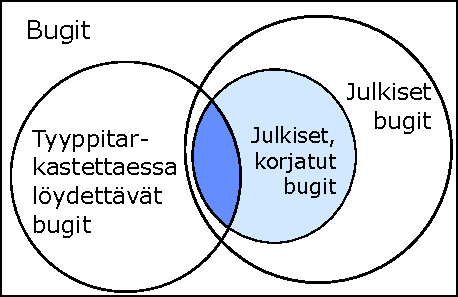
\includegraphics{images/to_type_or_not_to_type_venn.pdf}
\caption{To Type or Not to Type: Quantifying Detectable Bugs in JavaScript
         -tutkimuksen käsittelemät bugit\cite{ToTypeOrNotToType}.}
\label{fig:ToTypeOrNotToType}
\end{figure}

Kuvaajan \ref{fig:ToTypeOrNotToType} esittämässä tilanteessa suuri osa
bugeista ei ole julkisia, eli kehittäjät eivät ole havainneet bugia eivätkä
käyttäjät ole ilmoittaneet sellaisesta. Esimerkiksi seuraavanlainen koodi
saattaisi aiheuttaa vaikeasti havaittavan virheen, joka jäisi dynaamisessa
testaamisessa huomaamatta:

\begin{minipage}{\linewidth}
\begin{lstlisting}[caption={Vaikeasti havaittavan virheen aiheuttava koodiesimerkki}]
if (viikonpaiva === "perjantai") {
  // Alennus perjantaisin 5 euroa
  ostoskori.lisaaTuote({ nimi: "astiasto", Hinta: 10 });
} else {
  ostoskori.lisaaTuote({ nimi: "astiasto", hinta: 15 });
}
\end{lstlisting}
\end{minipage}
Esimerkin koodi ei toimi oikein perjantaisin, sillä \inlinecode{Ostos}-tyyppisen
objektin ominaisuus \inlinecode{hinta} on virheellisesti kirjoitettu isolla
alkukirjaimella. Koska bugi toistuu vain tietyissä olosuhteissa, se voi pysyä
havaitsemattomana pitkään. Staattiselle analyysille konditionaalisen ohjelman
tarkistaminen ei kuitenkaan ole ongelma ja tyyppiannotoituna kaikki kolme
työkalua pystyvätkin osoittamaan esimerkissä olevan virheen.

\section{Ohjelman optimointi käännösvaiheessa}
Aivan ensimmäiset tyyppijärjestelmät, kuten Fortranin staattinen tyypitys,
kehitettiin laskutoimitusten suoritusajan optimointia varten \cite{TypesAndProgrammingLanguages}.
Myös uudemmissa kielissä muuttujien tyypeistä saatavilla olevaa tietoa
voidaan käyttää ajonaikaisen turvallisuuden varmistavien tarkistusten
optimointiin.

Kun JavaScriptia optimoidaan käännösvaiheessa, on kuitenkin usein hyödyllistä
kiinnittää enemmän huomiota tuotetun koodin kokoon kuin suoritusaikaiseen
tehokkuuteen. Tyypillinen JavaScript-ohjelma ladataan sivulle saapuessa
internet-yhteyden yli juuri ennen suorittamista, minkä vuoksi ladattavan
koodin koon kasvattaminen minimaalisen suoritusajan edun vuoksi ei usein ole
kokonaisuudessaan hyödyllistä. Closure compiler on kehitetty erityisesti
JavaScript-koodin koon optimointia ajatellen. Muuttujanimet voidaan helposti
uudelleennimetä ilmankin staattisen tyypityksen apua, mutta sen lisäksi myös
joukko muita koodia keventäviä optimointeja on käytettävissä kun kääntäjällä
on muuttujien tyypeistä saatava tieto käytettävissä. Closure kääntäjä osaa
uudelleennimetä myös luokkamuuttujien nimiä lyhyemmiksi, poistaa
käyttämätöntä koodia, sekä function inlining.

\section{Tyyppimäärittelyt dokumentaationa}
Eksplisiittisesti kirjoitetut tyypit sekä editorin antama tieto muuttujien
tyypeistä voi toimia myös aiemmin kirjoitetun koodin dokumentaationa ja
kuvauksena siitä, miten moduulia on tarkoitus käyttää. Nykyaikasten editorien
vakio-ominaisuuksiin kuuluu kirjoittamisen tukeminen automaattisilla ehdotuksilla.
Ehdotukset nopeuttavat pitkien metodinimien kirjoittamista ja toimivat
eräänlaisena dokumentaation lähteenä, sillä ohjelmoija voi tutkia luokan tai
paketin tarjoamaa sisältöä ehdotettuja nimiä selaamalla. Automaattisia ehdotuksia
on mahdollista tarjota myös dynaamisesti tyyppitarkastetuille kielille, mutta
koodipohjan kasvaessa ja muuttuessa monimutkaisemmaksi ehdotusten tarkkuus
on vaikea pitää samalla tasolla kuin staattisesti tyypitetyissä kielissä.
Huonoimmillaan ehdotetut muuttuja- ja metodinimet valitaan yksinkertaisesti
listaamalla avoimista tiedostoista löytyviä nimiä, välittämättä sen
enempää siitä onko nämä metodit määritetty juuri kyseiselle tyypille.
Edistyneemmät ehdotusmoottorit kuten Visual Studiossa käytetty IntelliSense,
suorittavat osaa JavaScript-koodista taustalla ja analysoivat siten muuttujien
tyyppejä ajonaikana \cite{PreviewingSalsa, JavaScriptIntellisense}.
Tämä tekniikka yhdistettynä tavanomaisempaan tyyppien
käännösaikaiseen päättelyyn voi riittää tarjoamaan melko kattavan kuvauksen
jonkin muuttujan tyypistä, mutta jää silti jälkeen siitä tarkkuudesta jonka
IntelliSense osaa antaa TypeScriptillä kirjoitetulle koodille.
\begin{figure}
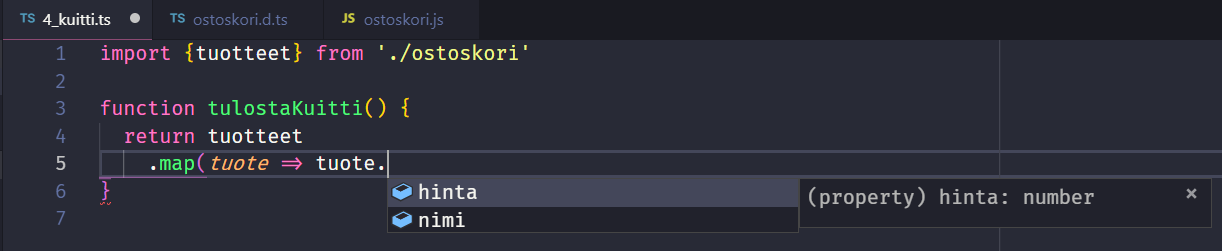
\includegraphics[width=0.5\textwidth]{images/intellisense_typescript}
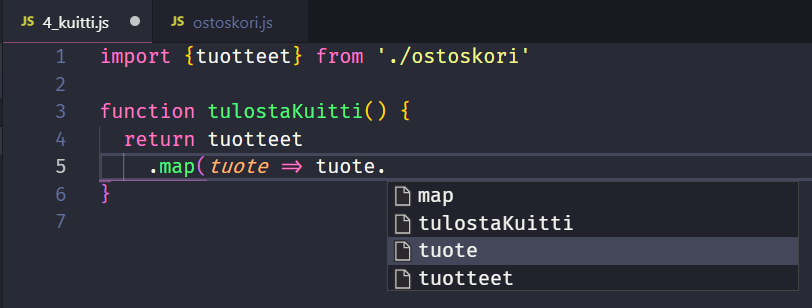
\includegraphics[width=0.5\textwidth]{images/intellisense_javascript}
\noindent
\caption{IntelliSensen tarjoamat ehdotukset TypeScriptille (vasemmalla) ja JavaScriptille (oikealla).}
\end{figure}
Automaattisten ehdotusten vaikutuksesta ohjelmointityön tehokkuuteen ei
kuitenkaan ole yleisesti hyväksyttyä, tutkittua varmuutta. Vaikka metodien
nimet olisivatkin ohjelmoijan nähtävillä editorissa, ne eivät välttämättä
sellaisenaan tarjoa tarpeeksi hyötyä dokumentaationa jotta työtehokkuus
kasvaisi merkittävästi. Vuonna 2015 toteutettu tutkimus
``An Empirical Investigation of the Effects of Type Systems and Code Completion
on API Usability using TypeScript and JavaScript in MS Visual Studio''
testasi staattisen tyypityksen ja automaattisten ehdotusten tehokkuutta
antamalla osallistujille toteutettavaksi ohjelmointitehtävän JavaScriptillä
ja TypeScriptillä, automaattisten ehdotusten kanssa ja niitä ilman
\cite{EmpiricalInvestigationOfCodeCompletion}. Tuloksissa ei näkynyt
tilastollisesti merkittävää eroa automaattisten ehdotusten kätyön ja niiden
käyttämättä jättämisen välillä, vaikka TypeScriptiä käyttäneet suoriutuivatkin
tehtävästä muista syistä JavaScriptiä käyttäneitä tehokkaammin.
  \chapter{Ongelmat JavaScriptin staattisessa tyypittämisessä}

\section{Luotettavuus, täydellisyys ja käytännöllisyys}

\begin{figure}
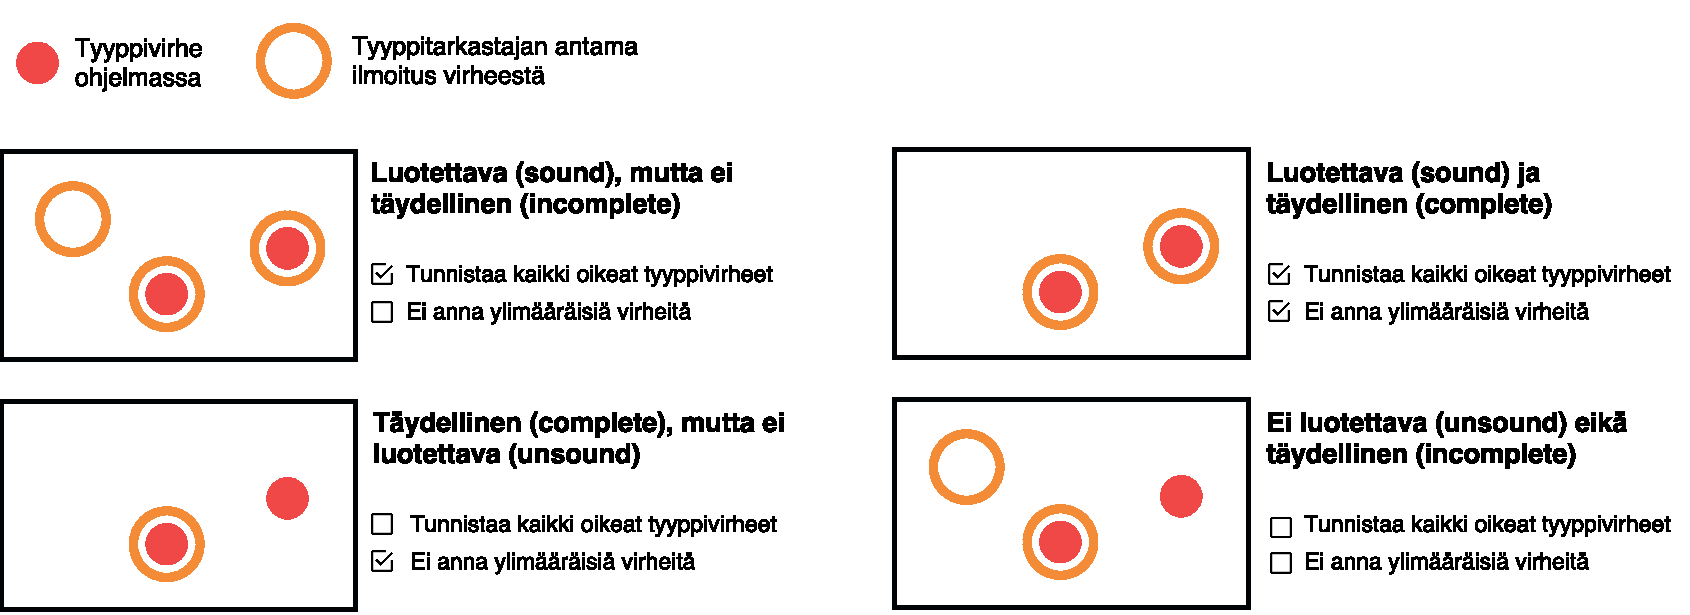
\includegraphics[width=\textwidth]{images/soundness_completeness2.pdf}
\caption{Tyyppijärjestelmän luotettavuus ja täydellisyys}
\end{figure}

Tyyppijärjestelmän luotettavuus (soundness) kuvaa sitä, kuinka suuren osan
mahdollisista ohjelmointivirheistä se estää. Täysin luotettava (sound)
tyyppijärjestelmä estää kaikki sellaiset virheet jotka sen on tarkoitus
estää \cite{CSE_ProgrammingLanguages}. Täydellisyys (completeness)
puolestaan kertoo salliiko tyyppijärjestelmä kielen sellaiset ominaisuudet
jotka eivät olisi ajonaikana tyyppivirheitä \cite{TypesAndProgrammingLanguages, CSE_ProgrammingLanguages}.

Jotta JavaScriptiä analysoiva tyyppijärjestelmä olisi luotettava, sen on
annettava virhe esimerkiksi seuraavasta ohjelmasta:

\begin{minipage}{\linewidth}
\begin{lstlisting}[caption={Virheellinen JavaScript-ohjelma: Lisätyllä tuotteella ei ole nimeä.}]
function osta(ostos) {
  lisaaTuote({
    nimi: ostos.nimi,
    hinta: ostos.hinta
  });
}

osta({ nimi: 'juusto', hinta: 5 });
osta({ hinta: 5 });
\end{lstlisting}
\label{fig:soundness_test}
\end{minipage}

Toisaalta jotta JavaScriptiä analysoiva tyyppijärjestelmä olisi täydellinen,
sen on sallittava tämä korjattu versio ylläolevasta ohjelmasta:

\begin{minipage}{\linewidth}
\begin{lstlisting}[caption={Toimiva JavaScript-ohjelma: Virheelliseltä kutsulta on suojauduttu tarkistuksella.}]
function osta(ostos) {
  if (typeof ostos.nimi === 'string') {
    lisaaTuote({
      nimi: ostos.nimi,
      hinta: ostos.hinta
    });
  }
}

osta({ nimi: 'juusto', hinta: 5 });
osta({ hinta: 5 });
\end{lstlisting}
\label{fig:completeness_test}
\end{minipage}

Esimerkit \ref{fig:soundness_test} ja \ref{fig:completeness_test} toimivat
odotetulla tavalla Flow:ssa. TypeScript vaatii eksplisiittisen tyyppiannotaation
osta-funktiolle, mutta toimii muuten samalla tavalla.


  \chapter{Yhteenveto}

Tyyppijärjestelmä on tärkeä ohjelmointikielen ominaisuus, jolla on suuri
vaikutus ohjelmistokehittäjän käyttökokemukseen.
Liian tiukka tyyppijärjestelmä voi rajoittaa sitä mitä kielellä voi tehdä,
sillä harva tyyppijärjestelmä on täydellinen (engl. complete).
Ohjelmointikielissä on usein ominaisuuksia joissa esimerkiksi merkkijonon
odotettu arvo on riippuvainen ohjelman rajapinnoista ja suoritusaikaisista
rakenteista, mutta joita tutkielmassa esitetyt tekniikat tai
monimutkaisemmatkaan tyyppijärjestelmät eivät välttämättä kykene
kuvaamaan ja tarkistamaan.

Lisäksi eksplisiittiset tyyppimäärittelyt vaativat lisää kirjoitettavaa
koodia kun funktioiden parametrien ja luokkien jäsenmuuttujien tyyppikuvaukset
tulee kirjoittaa kommentteihin (Closure) tai tyyppiannotaatioiksi
(TypeScript ja Flow).
Eksplisiittisistä tyyppimäärittelyistä voi olla hyötyä
koodin dokumentaationa, mutta kehittäjä saattaa myös kokea niiden
kirjoittamisen rasitteena. Dynaamisesti tyypitettyä koodia on usein
nopeampi tuottaa ja iteroida etenkin kehitysprosessin alkuvaiheissa, jolloin
käytettyjen tyyppien rakenne voi muuttua useaan kertaan. 

Dynaamisesti tyypitetyn koodin nopeasta kirjoitustahdista saatavat hyödyt jäävät kuitenkin
vähäisiksi jos lopputuotos ei toimi odotetulla tavalla. Ohjelmistovirheet heikentävät
käyttäjien tyytyväisyyttä ohjelmaan ja voivat pahimmillaan aiheuttaa
pysyvää vahinkoa saadessaan ohjelman toimimaan virheellisesti.
Staattinen tyypitys ohjaa kirjoitettua koodia turvalliseen suuntaan kehitysvaiheen alusta
loppuun ja torjuu tietynlaisia ohjelmointivirheitä tehokkaammin kuin
esimerkiksi ajonaikaista käyttäytymistä testaavat yksikkötestit.

Tässä tutkielmassa on esitelty kolme työkalua, jotka lisäävät dynaamisesti
tyypitettyyn JavaScriptiin käännösaikaisen tyyppitarkastuksen sekä syntaksin
tyyppien eksplisiittiseen määrittämiseen. Flow, TypeScript ja Closure
sallivat asteittaisen siirtymisen dynaamisesti tyyppitarkastetusta staattisesti
tarkastettuun, sekä staattisen tarkastuksen ohittamisen niissä osissa koodia
joihin sitä olisi liian vaikeaa tai mahdotonta lisätä.
Samankaltaisuus ja yhteensopivuus jo ennestään suositun JavaScriptin kanssa
yhdistettynä tyyppiturvallisuuteen, koodin kirjoittamista helpottaviin
työkaluihin ja selkeämmin dokumentoituun koodiin ovat nostaneet erityisesti
TypeScriptin käytön nopeaan kasvuun.


  \bibliographystyle{thesis/unsrtf}
  \bibliography{bibliografia}
  
  % make sure pagecount is correct even if references overflow to a new page
  \pagebreak\addtocounter{page}{-1}
  \eofpages
  \appendices
  
  % create your appendix chapters with command \appchapter{some name} instead
  % of \chapter{some name} for the automagic page counting to work
  %\input{file name of appchapter xxx}
  %\input{file name of appchapter yyy}
  %\input{file name of appchapter zzz}
  %\input{and so on}
  
  \eofapppages


\end{document}
